    \documentclass[12pt,a4paper]{article}
  \usepackage[utf8]{inputenc}
  \usepackage{amsmath,amsthm,amssymb,array,xcolor,multicol,verbatim,mathpazo}
  \usepackage[normalem]{ulem}
  %\usepackage[pdftex]{graphicx}
  \usepackage{fullpage}
  \usepackage{indentfirst}
  %\usepackage{endfloat}
  %\usepackage{cleveref}
  \usepackage{authblk}
  \usepackage{natbib}
  \usepackage{nth}
  \usepackage{graphicx}
  \usepackage{subcaption}
  \usepackage{pdfpages}
  
  %Fonts Setup
  
  
  \usepackage{adjustbox,rotating}
  \usepackage{multirow}
  \usepackage{multicol}
  \usepackage{color}
  \usepackage{graphicx}
  
  \renewcommand{\rmdefault}{ppl} % rm
  %\linespread{1.5}        % Palatino needs more leading
  \renewcommand{\baselinestretch}{2.0}
%  \setlength{\parskip}{2.0}
  
  \usepackage[scaled]{helvet} % ss
  \usepackage{courier} % tt
  %\usepackage{euler} % mathf
  %new font
  %\usepackage{libertine}
  
  %Table packages
  \usepackage{booktabs,caption,float}
  \usepackage[flushleft]{threeparttable}
  \usepackage{adjustbox}
  %define proposition
  \newtheorem{theorem}{Theorem}
  \newtheorem{proposition}{Proposition}
  \newtheorem{corollary}{Corollary}
  \newtheorem{lemma}{Lemma}
  
  \DeclareMathOperator*{\argmax}{argmax}
  \DeclareMathOperator*{\argmin}{argmin}
  %Color
  \definecolor{hdf}{HTML}{145680}
  \usepackage[colorlinks=true,linkcolor=blue,citecolor=blue,urlcolor=blue]{hyperref}
  %
  %\usepackage{titlesec}
  \newcommand{\sectionbreak}{\clearpage}
  
  
  \usepackage[utf8]{inputenc}
  \usepackage{amsmath,amsthm,amssymb,array,xcolor,multicol,verbatim,mathpazo}
  \usepackage[normalem]{ulem}
  \usepackage{indentfirst}
  %\usepackage{endfloat}
  %\usepackage{cleveref}
  \usepackage{authblk}
  \usepackage{natbib}
  \usepackage{nth}
  \usepackage{graphicx}
  \usepackage{subcaption}
  \usepackage{pdfpages}
  \usepackage{enumitem}
  \usepackage{bm}
  %Fonts Setup
  
  \usepackage[a4paper,margin=1in]{geometry}
  \usepackage{adjustbox}
  \usepackage{multirow}
  
  \usepackage{siunitx}
  
  \renewcommand{\rmdefault}{ppl} % rm
  
  \usepackage[scaled]{helvet} % ss
  \usepackage{courier} % tt
  %\usepackage{euler} % mathf
  %new font
  %\usepackage{libertine}
  
  %Table packages
  \usepackage{booktabs,caption}
  \usepackage[flushleft]{threeparttable}
  \usepackage{adjustbox}
  %define proposition
  
  
  


%=============================
	
\title{Econometric Modeling of Nonstationary Regressors \vspace{2cm}}
\author{Ying Zhou}
\date{February \\ 2020}



\begin{document}
	\maketitle
	\begin{center}
		
		\vspace{3cm}
		{ Supervised by \\ Professor Jiti Gao \\ Dr Hsein Kew }
		
		\vspace{3cm}
		
	\end{center}
	
	\begin{center}
		
		
		{ Department of Econometrics and Business Statistics \\  Monash University}
		
		
	\end{center}
	
%	\newpage
%	
%	\tableofcontents
	
	\newpage
	\pagenumbering{arabic}
	
	%\section{Introduction}
Most econometric theories and models are based on the assumption that the time-series under consideration is stationary. Theoretical properties of econometric models under stationarity assumptions are now well established. However many economic and financial variables are highly persistent and nonstationary. In my research, both chapters deal with econometric models in the presence of nonstationary time series. The first chapter adopts a time-varying model to uncover the nonlinear cointegrating relationship in an empirical study. The second chapter focuses on parametric nonlinear predictive models with multivariate nonstationary regressors.
\\

%there are three chapters dealing with high persistent time series. The first one adopts a time-varying model to uncover the cointegration relationship, the second chapter focuses on nonlinear model with multivariate nonstationary variables, and the third one uses a dataset that displays a wide range of time series properties.%
	
{\LARGE Chapter 1 - Time-Varying Modeling of Fertility and the Tax Benefits}

\section{Introduction}
%	As an attempt to decelerate population decline, the United States taxation authority has introduced tax benefits for dependents since 1913 to provide families with subsidy for each new-born child. \cite{whittington1990fertility} modeled the effect that this subsidy has on fertility rate by the following equation:
%	
%	$\text{General Fertility Rate}_{t}$
%	\begin{equation}
%	\begin{aligned}
%	&= \beta_{0}+\beta_{1} \text {Tax Benefits }_{t}+\beta_{2} \text { Male\&Asset Income }_{t} \\ & \quad +\beta_{3} \text { Unemployment }_{t}+\beta_{4} \text { Infant Mortality }_{t}+\beta_{5} \text { Immigration }_{t} \\ &\quad +\beta_{6} \text { Female Wage }_{t}+\beta_{7} \text { Pill }_{t}+\beta_{8} \mathrm{WW2 }_{t}+\beta_{9} \text { Time Trend }_{t}+\epsilon_{t}
%	\end{aligned}
%	\end{equation}
%	
%	The dependent variable, general fertility rate, is defined as the birthrate per thousand women between the age of 15 and 44. Pill and WW2 are dummy variables, referring to the availability of birth control pills and World War II respectively. Various other economic and demographic variables are included. They affect birthrates by either changing the demand for children or influencing the supply of births.
%	
%	\cite{whittington1990fertility} found that every increase of \$100 in tax benefits is associated with an increase of 2.1 to 4.2 births. But this strong and robust magnitude of their estimate has then been challenged in many empirical studies. 
%	
%	\cite{crump2011fertility} revisited the analysis of \cite{whittington1990fertility}, updated the data series, and included new measurements of tax benefits. They found that the variables in the regression are highly persistent and are integrated of order one. Thus, analysis in \cite{whittington1990fertility} may suffer from the problem of spurious regression. They performed a variety of cointegration tests and found no evidence of a cointegrating relationship. Therefore, the long-term tax-fertility relationship may not hold, only a short-term response occurs with a two-year lag. 
%	
%	However, the impact tax benefits has on fertility rate may not be constant. Along with the increasing costs of raising children, the fertility desire is going down even if the real tax benefits are going up. In another word, the fertility response to tax benefits can be varying in a different time period. Hence, traditional parametric models may be inadequate in capturing the possible hidden relationship.
%	
%	In our study, we consider a time-varying semiparametric model to describe the evolving relationship. We find evidence that tax policies did boost fertility desire before 1940. But the tax regulations are continuously losing its influence and become ineffective in recent two decades. 

%\subsection{Economic Background}
The governments of many countries, including the U.S., Germany, Canada and
Singapore, believe that they can influence fertility rates through tax
incentives. These governments are concerned with population decline and have
thus implemented a tax incentive that may directly affect the decision to
have a child. In the U.S., the personal exemption (PE, hereafter) for
dependent is an ongoing support item in the federal income tax system for
low-income households with children. The PE is designed as a public policy to lower the burden of taxation because the parents of each child receive this tax subsidy every year until the child reaches the age of 18.

It is apparent that the PE encourages fertility by lowering the cost of
children via tax relief. But, the question is: how much of an effect (if
any) did the changes in PE have on fertility? To answer the question, consider, for simplicity, the
following basic fertility model that describes the relationship between PE
and fertility rate:%
\[
\text{gfr}_{t}=\beta _{0}+\beta _{1}\text{PE}_{t}+\theta _{1}\text{Pill}_{t}+\theta _{2}%
\text{WW2}_{t}+\epsilon _{t},
\]%
where gfr (denotes the general fertility rate) is the number of
children born to every 1000 women between the ages of 15 and 44, PE is the real
dollar value of the personal exemption in 2005 dollars. The variable Pill is a dummy
variable equal to one in years that the birth control pill has been widely
available, from 1963 onwards. The variable WW2 is a dummy variable equal to
one during World War II (1941-45). 

The variable of interest is PE and we expect $\beta _{1}>0$ because an
increase in the tax value of the PE leads to an increase in the demand for
children. In an article published in the \textit{American Economic Review }%
(AER)\textit{, }Whittington, Alm and Peters (1990, WAP hereafter)
were the first to attempt to estimate the responsiveness of fertility to
changes in PE, i.e. $\beta _{1}$. Using their dataset we plot gfr and PE
from 1913 to 2005 (annual frequency) in Figure 1.

\begin{figure}[h]
	\caption{General Fertility Rate (left) and Personal Exemption (right) }
	\centering
	\begin{subfigure}[b]{0.48\linewidth}
		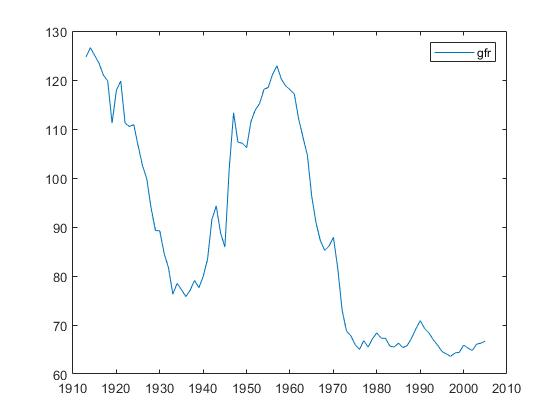
\includegraphics[width=\linewidth]{gfr.jpg}
	\end{subfigure}
	\begin{subfigure}[b]{0.48\linewidth}
	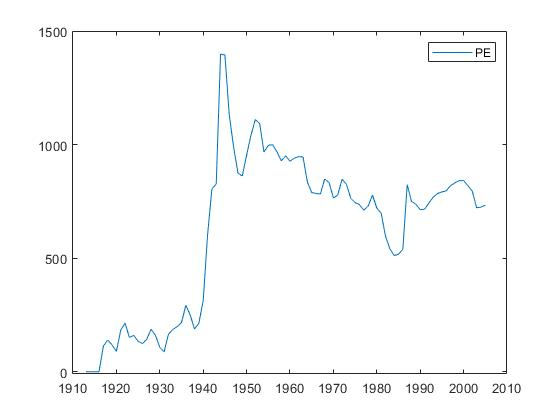
\includegraphics[width=\linewidth]{PE.jpg}
\end{subfigure}
\end{figure}

Figure 1 shows that the behavior of both the gfr and PE series appear to be nonstationary since they are not mean-reverting. In another article published in the AER,\textit{\ }Crump, Goda, Mumford (2011, CGM hereafter) revisit their traditional econometric modeling approach
because of the concern that gfr and PE may be spuriously correlated. Putting
aside the spurious regression issue, WAP control for other factors that
influence the birth decision by estimating the following model:%
\begin{eqnarray}
\text{gfr}_{t} &=&\beta _{0}+\beta _{1}PE_{t}+\beta _{2}\text{Male \& Asset Income}%
_{t}+\beta _{3}\text{Unemployment}_{t}  \label{bigModel} \\
&&+\beta _{4}\ \text{Infant Mortality}_{t}+\beta _{5}\text{Immigration}%
_{t}+\beta _{6}\text{Female Wage}_{t}  \nonumber \\
&&+\theta _{1}\text{Pill}_{t}+\theta _{2}\text{WW2}_{t}+\theta
_{3}t+\epsilon _{t}.  \nonumber
\end{eqnarray}
WAP use the sample period from 1913 to 1984 and find that $\hat{\beta}%
_{1}=0.017$ and significant at the 5\% level. Thus, a \$100 increase (in
2005 dollars) in the tax value of PE would increase the gfr by 1.7 births,
holding all other factors constant. CGM use a larger sample period from 1913
to 2005 and find that $\hat{\beta}_{1}=0.011$ and but significant at the
10\% level. Both of these results suggest that there is statistically
significant evidence of an effect of PE on birthrates. 

However, the regression in levels may produce spurious results due to the highly
persistent variables. To address this concern, CGM conduct a variety of cointegration tests. In the residual-based tests of \cite{arai2007testing}, they find no evidence to reject the null
hypothesis of cointegrating relationship. In the system based test of
\cite{saikkonen2000testing}, they also find, on balance, no evidence to
reject the null hypothesis of cointegrating relationships. Therefore, the empirical results reported in WAP suffer from the spurious regression problems. Indeed, CGM conclude that the specification presented in the original AER paper is not valid because there is no evidence of a meaningful long-run relationship.

There are of course a number of other studies, in addition to WAP and CGM
just mentioned, which investigate the effect of tax incentives on
birthrates. One set of studies explains that the significant and large
magnitude of fertility response do exist, but only in certain countries. For
example, using data from Quebec \cite{milligan2005subsidizing} find a large and significant effect. \cite{cohen2013financial} find strong impact of tax incentives
on fertility in Israel. 

Another set of studies finds that the impact of tax incentives depends on the race of the mother and  household income. For example, \cite{baughman2003did} claim that tax incentives only have a small positive effect for married non-white women. \cite{riphahn2017fertility} analyse the 1996 reform of the German child benefit program and find that couples from lower-income households tend to respond to tax incentives.  

In light of the evidence presented in CGM that there is lack of a cointegrating relationship, we examine whether there is instability in the time-series relationship between gfr and PE. We address this question by investigating the time-varying nature of this relationship and we do so by relaxing the assumption of constant coefficients in the fertility model given in (\ref%
{bigModel}). If it is found that the coefficients in the cointegration model
are time-varying, then this implies the existence of a nonlinear cointegrating relationship between gfr and PE. We are then able to examine the impact of PE on fertility. Accordingly, in this chapter, we are primarily interested in the extent to which the instability in the time-series relationship alters the conclusion of no linear cointegration. 

In a related literature on nonlinear cointegration, Breitung (2001) shows
that ignoring the nonlinear nature of the cointegrating relationship may
potentially lead to misleading conclusions about the absence of a meaningful long-run relationship. Martin (2000) to write more about Gael's paper here. 

In the next section, we describe the nonlinear cointegration model with time-varying coefficients and elaborates on the estimation methodology.  

\section{Nonlinear Cointegration Model and Estimation}
%\subsection{Model Specification and Estimation}

Phillips, Li and Gao (2017) propose the following nonlinear cointegration
model with time-varying coefficient functions:%
\begin{eqnarray}
y_{t} &=&x_{t}^{\prime }\beta _{t}+\epsilon _{t},\ \ \ t=1,...,T,
\label{NLcoint} \\
x_{t} &=&x_{t-1}+u_{t}  \nonumber
\end{eqnarray}%
where $\beta _{t}=\beta \left( \tau _{t}\right) ,\tau _{t}=t/T$ with $\beta \left(
.\right) $ is a $d$-dimensional vector of time-varying coefficients, $x_{t}$ is a $d$%
-dimensional $I\left( 1\right) $ processes, $u_{t}$ is a martingale
difference sequence and $\epsilon _{t}$ is an error term. This is a fully
nonparametric model because $\beta _{t}=\left( \beta _{1,t},...,\beta _{d,t}\right)
^{\prime }$ is an unknown function
of time. 

We can use this model to investigate the time-varying nature of the
cointegrating relationship between $y_{t}$ and $x_{t}$ -- in particular, whether we find the relationship has strengthened and/or weakened over time. Note that this model nests, as a special case, the commonly used linear cointegration model.  

We extend the nonlinear cointegration model (\ref{NLcoint}) to allow for
some coefficients to be constant over time instead of time-varying because
the empirical model of fertility involves two dummy variables (Pill and WW2) and a time trend variable.
The coefficients of these variables should not be time-varying. We therefore consider a semi-parametric nonlinear cointegration model of the form:%
\begin{equation}
y_{t}=x_{t}^{\prime }\beta \left( \tau _{t}\right) +z_{t}^{\prime }\theta+\epsilon _{t},  \label{semiPar}
\end{equation}%
where $z_{t}=\left( 1,Pill_{t},WW2_{t},t\right)^{\prime }$ and $\theta=\left(\theta_{1},...,\theta_{4}\right)^{\prime } $ is
an unknown parameter vector. 

The estimation method developed in Phillips, Li and Gao (2017) cannot be
used to estimate a semi-parametric model because it contains a non-parametric
part $\beta \left( .\right) $ and a parametric part $\theta .$ In many
semiparametric frameworks (see for example Fan and Huang (2005)), the
nonparametric part is estimated first and used to construct a parametric
estimator $\hat{\theta}$ in a multi-step estimation approach. We next present our three-step estimation procedure. 
%	We take three steps to estimate the unknown parameters $\beta(\tau)$ and $\theta$.
%	
%	\textbf{Step 1:} Assume that $\theta$ is known, model (3) can be written as:
%	$$
%	y_t - z_t^{\prime}\theta = x_t^{\prime} \beta(\tau_t) + \epsilon_{t}
%	$$
%	
%	When $\theta$ is known, the left hand side of the equation is already known to us. Therefore, the above equation has only one unknown parameter $\beta(\tau_t)$, which can be estimated by minimizing:
%	
%	$$
%	\underset{\theta}{\arg \min } \sum_{t=1}^{T}(y_t - z_t^{\prime}\theta - x_t^{\prime} \beta(\tau_t))^2 K(\dfrac{\tau_t - \tau}{h})
%	$$
%	where K($\cdot$) is a kernel function and h is the bandwidth.
%	%? specify the form of k? how we choose h? 
%	
%	We can then obtain the estimated $\beta$ denoted by $\bar{\beta}(\tau,\theta)$.
%	
%	\textbf{Step 2:}
%	Once $\beta$ is known, in model (3), we can get the estimation of $\theta$. Put $x_{t}^{\prime} \beta\left(\tau_{t}\right)$ to the left hand side of the model, we can estimate $\theta$ based on an asymptotic model of the form, where $\theta$ is the only unknown parameter:
%	
%	$$
%	y_t - x_t^{\prime} \bar{\beta}(\tau_t,\theta) = z_t^{\prime}\theta + \epsilon_{t}
%	$$
%	
%	Minimizing:
%	
%	$$
%	\underset{\theta}{\arg \min } \sum_{t=1}^{T}(y_t - z_t^{\prime}\theta - x_t^{\prime} \bar\beta(\tau_t))^2
%	$$
%	
%	The least-square estimator of $\theta$ is then given by:
%	\begin{equation*}
%	\hat{\theta} = \left(\sum_{t=1}^{T} \bar{z_t}\bar{z_t}^{\prime}\right)^{-1} \left(\sum_{t=1}^{T} \bar{z_t} \bar{y_t}\right)
%	\end{equation*}
%	where 
%	$$ \bar{z_t} = z_t - x_t^{\prime} \left(\sum_{t=1}^{T} x_t^{\prime} x_t K(\dfrac{\tau_{t} - \tau}{h}) \right)^{-1}\sum_{t=1}^{T} K(\dfrac{\tau_{t} - \tau}{h}) x_t z_t^{\prime}$$
%	
%	$$\bar{y_t} = y_t - x_t^{\prime} \left(\sum_{t=1}^{T} x_t^{\prime} x_t K(\dfrac{\tau_{t} - \tau}{h}) \right)^{-1}\sum_{t=1}^{T} K(\dfrac{\tau_{t} - \tau}{h}) y_t x_t$$
%	
%	\textbf{Step 3:} As we have already estimated $\bar{\beta}(\tau,\theta)$, we can get the estimated $\hat{\beta}$ by plugging in $\hat{\theta}$ we obtained in step 2. $\hat{\beta}$ is estimated as:
%	\begin{equation*}
%	\begin{aligned}
%	\hat{\beta}\left(\tau\right) &=\bar{\beta}\left(\tau_{t} ; \hat\theta\right)\\ &=\left[\sum_{t=1}^{T} x_{t} x_{t}^{\prime} K\left(\frac{\tau_{t}-\tau}{h}\right)\right]^{-1} \cdot \sum_{t=1}^{T} K\left(\frac{\tau_{t}-\tau}{h}\right) \cdot\left(y_{t} x_t - x_t z_{t}^{\prime} \hat\theta\right)
%	\end{aligned}
%	\end{equation*}
%	


Step 1: To concentrate only on estimating the non-parametric component, we re-write the above model as follows
\[
y_{t}-z_{t}^{\prime }\theta =x_{t}^{\prime }\beta \left( \tau \right) +\varepsilon _{t}. 
\]%
It is now clear that the right-hand-side of this equation contains only the parameter of interest $\beta \left(.\right) $. Let $\theta $ be given at this stage. Then, this becomes a fully non-parametric model and hence we can apply the usual non-parametric estimation method. We estimate $\beta \left( \tau \right) $ by $%
\mu $ such that we minimise 
\[
\sum_{t=1}^{T}\left( y_{t}-z_{t}^{\prime }\theta -x_{t}^{\prime }\mu \right)
^{2}K\left( \frac{\tau _{t}-\tau }{h}\right), 
\]%
where $K\left( .\right) $ is a kernel function and $h$ is the bandwidth. In practice, the bandwidth can be chosen as $h=0.3T^{-1/5}$. In
this case, $\beta \left( \tau \right) $ can be initially estimated by 
\[
\bar{\beta}\left( \tau \right) =\bar{\beta}\left( \tau ,\theta \right)
=\left( \sum_{t=1}^{T}x_{t}x_{t}^{\prime }K\left( \frac{\tau _{t}-\tau }{h}%
\right) \right) ^{-1}\sum_{t=1}^{T}K\left( \frac{\tau _{t}-\tau }{h}\right)
\left( y_{t}-z_{t}^{\prime }\theta \right) x_{t}. 
\]

Step 2: We estimate $\theta $ by minimising 
\[
\sum_{t=1}^{T}\left( y_{t}-z_{t}^{\prime }\theta -x_{t}^{\prime }\bar{\beta}%
\left( \tau _{t},\theta \right) \right) ^{2} 
\]%
over $\theta $ to obtain a least squares estimator $\hat{\theta}$ as%
\[
\widehat{\theta}=\left(\sum_{t=1}^{T} \bar{z}_t\bar{z}_t^{\prime}\right)^{-1} \left(\sum_{t=1}^{T} \bar{z}_t \bar{y}_t\right), 
\]%
where%
\[
\bar{z}_{t}= z_t - x_t^{\prime} \left(\sum_{s=1}^{T} x_s x_s^{\prime}  K(\dfrac{\tau_{s} - \tau_t}{h}) \right)^{-1}\sum_{s=1}^{T} K(\dfrac{\tau_{s} - \tau_t}{h}) x_s z_s,
\]%
and%
\[
\bar{y}_{t}= y_t - x_t^{\prime} \left(\sum_{s=1}^{T} x_s x_s^{\prime} K(\dfrac{\tau_{s} - \tau_t}{h}) \right)^{-1}\sum_{s=1}^{T} K(\dfrac{\tau_{s} - \tau_t}{h}) x_s y_s.
\]

Step 3. We re-estimate $\beta \left( \tau \right) $ by plugging in $\widehat{\theta}$ to define $\widehat{\beta}\left( \tau \right) =\bar{\beta}\left( \tau ,\widehat{\theta}\right)$. 

%	To estimate parameters in model (3), we first assume that $\beta$ is known, thenthe least square estimator of $\theta$ is:
%	\begin{equation}
%	\hat{\theta} = \left(\sum_{t=1}^{T} \bar{z_t}\bar{z_t}^{\prime}\right)^{-1} \left(\sum_{t=1}^{T} \bar{z_t} \bar{y_t}\right)
%	\end{equation}
%	
%	where 
%	
%	$$\bar{z_t} = z_t - x_t^{\prime} \left(\sum_{t=1}^{T} x_t^{\prime} x_t K(\dfrac{\tau_{t} - \tau}{h}) \right)^{-1}\sum_{t=1}^{T} K(\dfrac{\tau_{t} - \tau}{h}) x_t z_t^{\prime}$$
%	
%	$$\bar{y_t} = y_t - x_t^{\prime} \left(\sum_{t=1}^{T} x_t^{\prime} x_t K(\dfrac{\tau_{t} - \tau}{h}) \right)^{-1}\sum_{t=1}^{T} K(\dfrac{\tau_{t} - \tau}{h}) y_t x_t$$
%	
%	and K($\cdot$) is a kernel function, h is bandwidth selected by the degree of smoothing. 
%	
%	Then the time-varying parameter $\beta$ can then be estimated as:
%	\begin{equation}
%	\bar{\beta}\left(\tau_{t}\right)=\bar{\beta}\left(\tau_{t} ; \hat\theta\right)=\left[\sum_{t=1}^{T} x_{t} x_{t}^{\prime} K\left(\frac{\tau_{t}-\tau}{h}\right)\right]^{-1} \cdot \sum_{t=1}^{T} K\left(\frac{\tau_{t}-\tau}{h}\right) \cdot\left(y_{t} x_t - x_t z_{t}^{\prime} \hat\theta\right)
%	\end{equation}
\subsection{Confidence Interval}

For samples that are drawn from normal distribution, confidential interval is calculated by plugging values into the following equation:
$$\left(\bar{x}-t_c \frac{s}{\sqrt{T}}, \bar{x}+t_c \frac{s}{\sqrt{T}}\right),$$
where $\bar{x}$ is the sample mean, $s$ is the sample variance and $t_c$ is the critical value taken from the student's t distribution. However, the limiting distributions of the semi-parametric estimators introduced in the previous subsection have yet to be established. Therefore, confidence interval cannot be constructed based on the asymptotic variance of the estimator. Instead, we adopt a bootstrap method.

In our semi-parametric model, confidential interval for the time-varying coefficients are constructed using a wild bootstrap method originally proposed by \cite{liu1988bootstrap} and \cite{mammen1993bootstrap}. Wild bootstrap is a special case of residual bootstrap, which draws the errors independent from the empirical distribution of the residuals. We adopt a residual bootstrap method, because in the regression model
$$
y_t = x^{\prime}_{t}\beta(\tau_{t}) +z_t^{\prime}\theta +\epsilon_t,
$$
there is a conditional mean restriction, ie. $\mathbb{E}\left(\epsilon_{t} | \boldsymbol{x}_{t}\right)=0$. Thus a normal bootstrap which samples from the original observations ($y^{*}_t$,$x^{*}_t$,$z^{*}_t$) does not satisfy this restriction. 

To conduct the residual bootstrap, we hold the regressors $x_t$ fixed, then draw the errors $\epsilon^{*}_t$  by using auxiliary random variables $\eta^{*}_t$: \, $\epsilon_{t}^{*}=\widehat{\epsilon}_{t} \eta_{t}^{*}$.We then adopt a two-point distribution structure for $\eta$ as suggested by \cite{mammen1993bootstrap}:
$$\begin{array}{l}
\mathbb{P}\left(\eta_{t}^{*}=\frac{1+\sqrt{5}}{2}\right)=\frac{\sqrt{5}-1}{2 \sqrt{5}}  \ \ \ \mbox{and} \ \ \ \mathbb{P}\left(\eta_{t}^{*}=\frac{1-\sqrt{5}}{2}\right)=\frac{\sqrt{5}+1}{2 \sqrt{5}}.
\end{array}$$

Then, $y^{*}_i$ can be generated by:
$$
y_{t}^{*}=x^{\prime}_{t}\hat\beta(\tau_{t}) +z_t^{\prime}\widehat{\theta}+ \epsilon_{t}^{*}.
$$

And the bootstrap estimator $\widehat{\beta}^{*}(\tau)$ can be estimated using ($y^{*}_t$,$x^{*}_t$, $z^{*}_t$). The choice of the two-point distribution for $\eta$ ensures that the central moment of $\widehat{\beta}^{*}(\tau)$ matches the first three central moment of $\widehat{\beta}(\tau)$, therefore, the percentile-$t$ interval and one-sided $t$--tests achieve the asymptotic distribution. 
%	This scheme has the advantage that it retains the information in the explanatory variables.
%	
%	The idea of this wild bootstrap is to leave the regressors at their sample value, but to resample the response variable based on the residual values. That is, for each replicate, one computes a new dependent variable y based on:
%	$$
%	y_i^{*} = \hat{y_i} +\hat{\epsilon_{i}}v_i
%	$$ 
%	
%	Different forms are used for the random variable $v_i$. In our research we adopt a distribution suggested by Mammen (1993). 
The procedure for constructing the point-wise confidence intervals for the time-varying coefficients using the wild bootstrap is outlined as follows:
\begin{enumerate}
	\item Estimate $\beta(\tau)$ and $\theta$ by the estimation method introduced in the previous section, and obtain the estimators $\widehat{\beta}(\tau)$ and $\widehat{\theta}$, respectively.
	
	\item Let $\hat{\epsilon_{t}}$ = $y_t - x_t^{\prime} \widehat{\beta}(\tau_{t})  - z^{\prime}\widehat{\theta}$. Generate the bootstrap residuals {$\epsilon_{t}^*$} by   $\hat{\epsilon_{t}}\eta_t^*$, where {$\eta_t^*$, 1 $\leq$ t $\leq$ T} is a sequence of i.i.d random variables drawn from a two-point distribution:
	$$
	P\left(\eta_{1}^{*}=\frac{-(\sqrt{5}-1)}{2}\right)=\frac{\sqrt{5}+1}{2 \sqrt{5}} \text { and } P\left(\eta_{1}^{*}=\frac{\sqrt{5}+1}{2}\right)=\frac{\sqrt{5}-1}{2 \sqrt{5}}.
	$$
	
	\item  Generate $y_{t}^{*}=\widehat{\beta}^{\prime}(\tau_t) x_{t} + z^{\prime}\widehat{\theta} +\epsilon_{t}^{*}$. Then use the data set $\left\{\left(x_{t}, z_{t}, y_{t}^{*}\right), 1 \leq t \leq T\right\}$ to re--estimate $\hat{\beta}(\tau)$. Denote the resulting estimate by $\widehat{\beta}^*(\tau)$.
	
	\item Repeat step 2 and 3 B= 250 times to obtain B bootstrap samples, $\widehat{\beta}_i^*(\tau)$, for $i = 1,..., B$. The estimate of the standard deviation, denoted by SD($\widehat{\beta}(\tau)$), is the sample standard deviation of $\left\{\widehat{\beta}^{*}(\tau), for \quad i=1, \ldots, B\right\}$. Denote the resulting estimate as $SD^*(\widehat{\beta}(\tau))$.
	
	\item Use the critical value $c_{\alpha / 2} = 1.96$ from the standard normal distribution. The $95\%$ confidence interval of $\beta(\tau)$ is constructed by $\widehat{\beta}(\tau) \pm 1.96 \times \operatorname{SD}^{*}\left(\widehat{\beta}(\tau)\right)$.
\end{enumerate}

Using the estimation technique developed in this section, we next examine the time-series relationship between gfr and PE. 


\section{Empirical Results}

	\cite{crump2011fertility} 
	
	
	included two additional measurements, child tax credit (denoted as CTC) and the earned income tax credit (denoted as EITC) to the total child subsidy series. Both of these two new subsidies affect birth decisions through its impact on the opportunity cost of having a child. Higher tax benefits are expected to increase the general fertility rate. In our analysis, the primary variable of interest is the real value of tax benefits for dependents, which is a combination of PE, CTC and EITC.
	
\subsection{Nonlinear Cointegration Model with Time-varying Coefficients}
%	
%	\subsubsection{Time-varying Coefficient}
%	Using the estimation procedure, the time-varying effects of tax benefits have on general fertility rate are shown in figure 1. Different from the constant ordinary least square result at the level of 0.02 (2 more births with an \$100 increase in personal exemption), figure 1 shows that tax benefits have a decreasing impact on general fertility rate. 
%	
%	Before WWII, a \$100 increase in tax benefit would increase general fertility rate by 5 births. This effect dropped from then on till 1980. After 1970, tax benefits almost have no impact on general fertility rate. 
%	\begin{figure}
%		\caption{Time-varying effect of tax benefit on general fertility rate}
%		\centering
%		\begin{subfigure}[b]{0.45\linewidth}
%			\includegraphics[width=\linewidth]{CI_new201.jpg}
%		\end{subfigure}
%		\begin{subfigure}[b]{0.45\linewidth}
%			\includegraphics[width=\linewidth]{CI_new301.jpg}
%		\end{subfigure}
%	\end{figure}

%Figure 2 shows the time-varying coefficient of personal exemption, $\beta_{1,t}$. Before World War II, the impact of personal exemption on general fertility rate was significant. Specifically, holding all other factors constant, a \$100 increase in personal exemption would increase the general fertility rate by more than 4 births in 1920. But this impact is diminishing over time and reached the lowest point of -0.02 around 1980. Although it rose moderately after 1980, the effect is still slightly negative around the year 2000. The result suggests that personal exemption lost its impact over time and is no longer an effective policy to boost fertility. 
%
%
%
%% add zero lines to these ones
%\begin{figure}[!htp]
%	\caption{Time-varying Coefficient of Personal Exemption}
%	\centering
%	\begin{subfigure}[b]{0.7\linewidth}
%		\includegraphics[width=\linewidth]{CI_new01.jpg}
%	\end{subfigure}
%\end{figure}
%
%Figure 4 shows the time-varying effect of noEITC, which is the second measurement of tax benefit. It started with a large and significant number in 1920, around 0.05, which indicates a \$100 increase in this tax benefit would increase the general fertility rate by 5 births. The effect went down quickly and became insignificant between 1940 and 1980. After 1980, as CTC has been included, the impact of tax benefit on fertility rate went up again and become significant around 2000. However, the magnitude is only 0.01, much lower than it was in 1920 and also lower than the number in \cite{whittington1989fertility}.
%
%
%\begin{figure}[!htp]
%	\caption{Time-varying Coefficient of noEITC}
%	\centering
%	\begin{subfigure}[b]{0.7\linewidth}
%		\includegraphics[width=\linewidth]{CI_new301.jpg}
%	\end{subfigure}
%\end{figure}
%
%Figure 5 presents the time-varying estimation of Subsidy, which includes all three tax incentives. It has a very similar pattern with noEITC. The only difference is that the effect of Subsidy became significant again before 1980 instead of after 1980 as in the case of noEITC measurement. All of the three tax benefit measurements indicate that although tax incentives helped the government to increase fertility rate before, the effectiveness of this policy need to be reconsidered now.
%
%\begin{figure}[!htp]
%	\caption{Time-varying Coefficient of Subsidy}
%	\centering
%	\begin{subfigure}[b]{0.7\linewidth}
%		\includegraphics[width=\linewidth]{CI_new201.jpg}
%	\end{subfigure}
%\end{figure}
%
%\subsubsection{The Existence of Long-run Relationship}
%To justify that our time-varying model specifications is valid, we need to confirm that there is a long-run relationship between tax benefits and general fertility rate. We first plot the residual sequence and its ACF plot. In Figure 2, the left panel shows the time series plot of residual sequence, while the right panel presents the corresponding ACF plot. It is clear that the residual sequence is stationary and the AR(1) coefficient is smaller than 0.6. 
%
%We then perform the augmented Dickey–Fuller (ADF) test on the residual sequence and find that the null hypothesis of a unit root can be rejected at 1\% level.
%
%Therefore, the plots and the stationary test result suggest that under our semi-parametric model specification, there exists a nonlinear cointegration. Then, we can conclude that there is a long-run relationship between tax benefit and fertility rate.
%
%\begin{figure}[!htp]
%	\caption{Plots and ACF Plots for Residual Sequences}
%	\centering
%	%		\begin{subfigure}[b]{0.45\linewidth}
%	%			\includegraphics[width=\linewidth]{et1.jpg}
%	%		\end{subfigure}
%	%		\begin{subfigure}[b]{0.45\linewidth}
%	%			\includegraphics[width=\linewidth]{acf_et1.jpg}
%	%		\end{subfigure}
%	%		\begin{subfigure}[b]{0.45\linewidth}
%	%			\includegraphics[width=\linewidth]{et2.jpg}
%	%		\end{subfigure}
%	%		\begin{subfigure}[b]{0.45\linewidth}
%	%			\includegraphics[width=\linewidth]{acf_et2.jpg}
%	%		\end{subfigure}
%	\begin{subfigure}[b]{0.45\linewidth}
%		\includegraphics[width=\linewidth]{et3.jpg}
%	\end{subfigure}
%	\begin{subfigure}[b]{0.45\linewidth}
%		\includegraphics[width=\linewidth]{acf_et3.jpg}
%	\end{subfigure}
%\end{figure}
%\pagebreak

We estimate the following nonlinear cointegration model with time-varying coefficients for the basic model of fertility.


\begin{equation}
\begin{aligned}
\text{gfr}_{t} &= \theta_{1}+\theta_{2} \text { Pill}_{t}+\theta_{3} \mathrm { WW2}_{t}+\theta_{4} \text { Time Trend }_{t} + \beta_{1,t} \text { Tax Benefits}_{t} \\ & \quad +\beta_{2,t} \text { Male \& Asset Income}_{t}  +\beta_{3,t} \text { Unemployment}_{t}+ \beta_{4,t} \text { Infant Mortality}_{t} \\ & \quad +\beta_{5,t} \text { Immigration}_{t} +\beta_{6,t} \text { Female Wage}_{t}+\epsilon_{t}, \label{tvmodel}
\end{aligned}
\end{equation}


In our empirical study, we estimate three regressions using different tax measurements but keep all the other independent variables in model (\ref{tvmodel}) unchanged. In the first regression (R1 hereafter), we use "Subsidy" as the tax benefits, which includes "PE + CTC + EITC". In the second regression (R2 hereafter), we use "noEITC" which includes "PE + CTC", while in the third one (R3 hereafter), we adopt PE. The time-varying semi-parametric model in our empirical study is shown below:

Figure 2 plots the time-varying (TV) coefficient for "Subsidy" as the variable for tax benefits, $\beta_{1,t}$ along with its 95\% confidence interval. It shows the evolution of response of general fertility rate to "Subsidy". Before World War II, the impact of subsidy on general fertility rate was significant according to the 95\% confidence intervals. Specifically, holding all other factors constant, a \$100 increase in personal exemption would increase the general fertility rate by more than 4 births in 1920. But this impact is diminishing over time and was not significant around 1980. Although it rose moderately after 1980, the effect is only slightly above zero around the year 2000. The result suggests that tax benefits lost its impact over time and is no longer an effective policy to boost fertility. 



% add zero lines to these ones
\begin{figure}[!htp]
	\caption{Time-varying Coefficient for Subsidy}
	\centering
	\begin{subfigure}[b]{0.7\linewidth}
		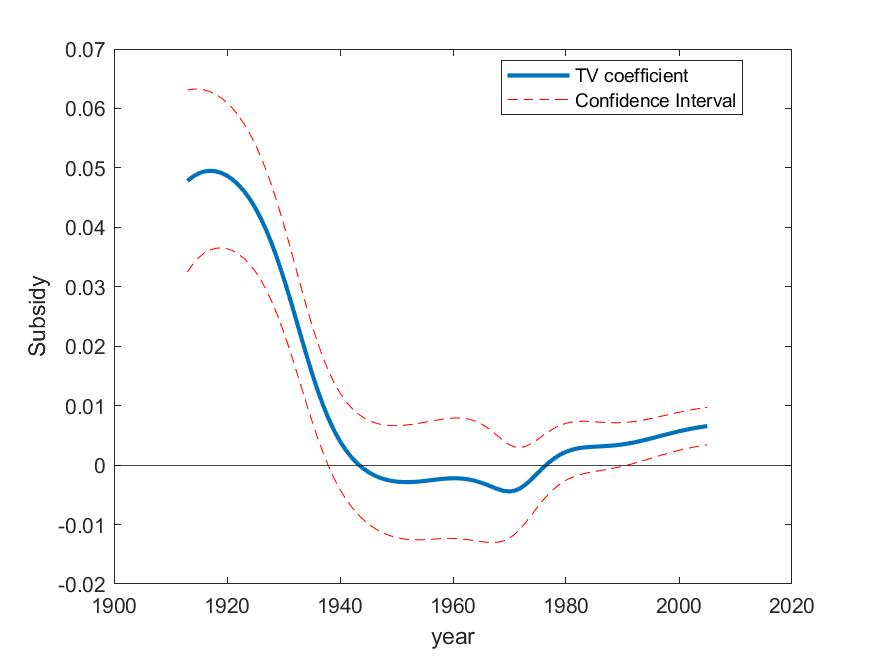
\includegraphics[width=\linewidth]{CI_n201.jpg}
	\end{subfigure}
\end{figure}

Figure 3 shows the time-varying effect of using noEITC as the variable for tax benefits. We observed very similar pattern in this cases. Figure 4 presents the time-varying estimation of personal exemption. The estimate of $\beta(\tau)$ start out positive and large. However, it drops to zero rapidly and remains low for the remainder of the sample period. 

%It started with a large and significant number in 1920, around 0.05, which indicates a \$100 increase in this tax benefit would increase the general fertility rate by 5 births. The effect went down quickly and became insignificant between 1940 and 1980. After 1980, as CTC has been included, the impact of tax benefit on fertility rate went up again and become significant around 2000. However, the magnitude is only 0.01, much lower than it was in 1920 and also lower than the number in \cite{whittington1990fertility}.

\begin{figure}[!htp]
	\caption{Time-varying Coefficient of noEITC and PE}
	\centering
	\begin{subfigure}[b]{0.7\linewidth}
		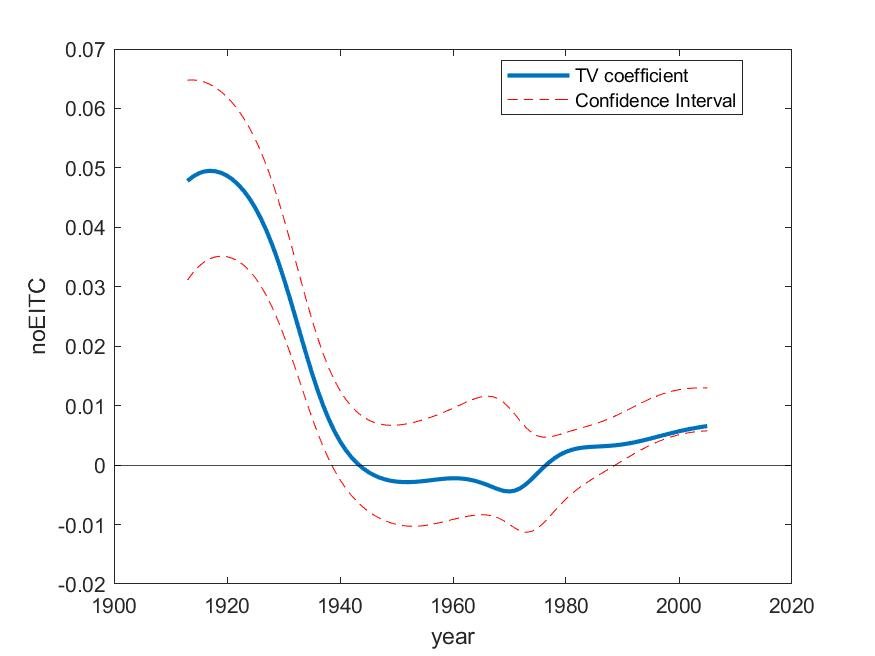
\includegraphics[width=\linewidth]{CI_n301.jpg}
	\end{subfigure}
\end{figure}


%	\begin{figure}
%		\caption{Time-varying effect of tax benefit on general fertility rate}
%		\centering
%		\begin{subfigure}[b]{0.45\linewidth}
%			\includegraphics[width=\linewidth]{CI_new201.jpg}
%		\end{subfigure}
%		\begin{subfigure}[b]{0.45\linewidth}
%			\includegraphics[width=\linewidth]{CI_new301.jpg}
%		\end{subfigure}
%	\end{figure}



%presents the time-varying estimation of personal exemption. It has a very similar pattern with noEITC. The only difference is that the effect of Subsidy became significant again before 1980 instead of after 1980 as in the case of noEITC measurement. All of the three tax benefit measurements indicate that although tax incentives helped the government to increase fertility rate before, the effectiveness of this policy need to be reconsidered now.

\begin{figure}[!htp]
	\caption{Time-varying Coefficient of Subsidy}
	\centering
	\begin{subfigure}[b]{0.7\linewidth}
		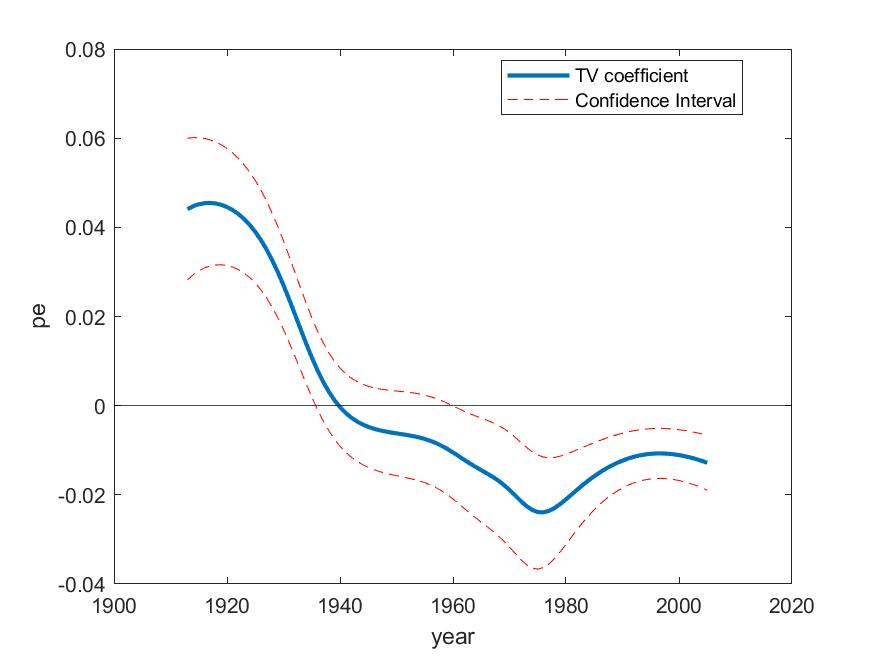
\includegraphics[width=\linewidth]{CI_n101.jpg}
	\end{subfigure}
\end{figure}


%\begin{figure}[p]
%    \caption{New Measurements of Tax Benefits}
%    \centering
%    \begin{subfigure}[b]{0.45\linewidth}
%        \includegraphics[width=\linewidth]{CI_new201.jpg}
%    \end{subfigure}
%    \begin{subfigure}[b]{0.45\linewidth}
%        \includegraphics[width=\linewidth]{CI_new301.jpg}
%    \end{subfigure}
%\end{figure}

%\subsubsection{Time-varying Effect of Other Variables}
%Coefficients for other independent variables also present time-varying features. Take R1 as example, the infant mortality rate had a negative impact on the fertility rate before 1980 (as shown in Figure 6). It increased sharply afterward but started to fall recently. But it always fluctuates around zero because it captures two possible effects. The high infant mortality rate may encourage the family to have more babies if people tend to maintain a certain family size. However, it also inclines to decrease the fertility rate as the cost of producing a healthy child rises. Therefore, when the previous effect dominants, infant mortality shows a positive impact on fertility rate, as between 1980 and 2000. 
%
%\begin{figure}
%	\caption{Time-Varying Coefficient Result}
%	\centering
%	\begin{subfigure}[b]{0.45\linewidth}
%		\includegraphics[width=\linewidth]{CI_new04.jpg}
%	\end{subfigure}
%	\begin{subfigure}[b]{0.45\linewidth}
%		\includegraphics[width=\linewidth]{CI_new05.jpg}
%	\end{subfigure}
%\end{figure}
%
%The coefficient of immigration also shows positive but time-varying property. Because fertility rate differs across cultures, when more immigrants from countries with higher birthrate come to the US, the fertility rate in US will increase. However, as the desire of having children is decreasing in most places of the world, the impact of the immigrant on the US fertility rate drops after 1960 although the total effect is still positive.
%
%In addition, the coefficients of two dummy variables, Pill and WWII, are both negative, which is consistent with our expectations. It means that the absence of young men during war time and the availability of birth control pills have negative effect on fertility rate. The results of dummy variables can be found in Appendix B.

% ? introduce the time trend and intercept
% How about all the other coefficients? put them into the appendix
% The pis don't look very well though...sad

%\subsection{Cointegration Test}

To justify that our time-varying model specifies a nonlinear cointegrating relationship between tax benefits and general fertility rate, we impose KPSS test on residuals sequences from three regression. Table 2 present the test results. In all three regressions, the residual sequences are stationary at 1\% level. Therefore, there is a cointegrating relationship between tax benefits and general fertility rate under our model specification.

% Table generated by Excel2LaTeX from sheet 'Sheet3'
\begin{table}[!htp]
	\centering
	\caption{KPSS Test of Residual Sequences}
	\begin{tabular}{llll}
		\toprule
		& \multicolumn{1}{c}{$\epsilon_{t}$ (R1)} & \multicolumn{1}{c}{$\epsilon_{t}$ (R2)} & \multicolumn{1}{c}{$\epsilon_{t}$ (R3)} \\
		\midrule
		Test Statistics & \multicolumn{1}{c}{0.1293} & \multicolumn{1}{c}{0.0885} & \multicolumn{1}{c}{0.0971} \\
%		\midrule
%		10\% Critical Value & \multicolumn{1}{c}{0.347} & \multicolumn{1}{c}{0.0885} & \multicolumn{1}{c}{0.0971} \\
		Conclusion & \multicolumn{1}{c}{Stationary} & \multicolumn{1}{c}{Stationary} & \multicolumn{1}{c}{Stationary} \\
		\midrule
		\multicolumn{4}{l}{\textit{\footnotesize{The critical value at 10\% is 0.347, therefore, we do not reject the null hypothesis of stationary.}}} \\
	\end{tabular}%
	\label{tab:addlabel}%
\end{table}%

\section{Conclusion and Future Research}
%We have examined the effect of tax policies on fertility rate by time-varying semiparametric model. Using yearly data from 1913 to 2015, our estimates reveal that the impact of tax policies is diminishing. In our future work, we will establish the asymptotic distributions of
%our estimators and discuss the asymptotic properties for both parametric and nonparametric components of our model.

Existing studies have found that the general fertility rate responds to tax benefits and this effect is statistically significant. However, these studies find no evidence of cointegration. It suggests that the regressions in levels may produce spurious results since the tax benefits and birth rates series are nonstationary. 

Our research fills this gap by specifying a semi-parametric time-varying model. We uncover the nonlinear cointegrating relationship between tax benefits and fertility rate by allowing the coefficients to be time-varying.

We present evidence suggesting that the impact that tax benefits have on fertility rate is diminishing over time and stays at a low level after 2000. Tax incentives used to be an effective policy instrument, but after World War II, the U.S. fertility rate is not responsive at all to child tax benefits. Even when new tax benefits, such as CTC and EITC are introduced, they are no longer an effective government policy to increase the fertility rate. Overall, this study improves our understanding of how tax incentives affect people's decision to have a child. It also suggests that in order to increase the fertility rate, the government may need to seek new policies other than tax benefits. 

In my future research, I plan to consider how the tax benefits at time t-1 or t-2 influences the general fertility rate t since \cite{whittington1990fertility} point out that it may take families one or two years to react to the change of tax benefits. Then, we will perform a hypothesis test to show the significance of the lagged tax benefits variables.

%$\text{General Fertility Rate}_{t}$
%\begin{equation*}
%\begin{aligned}
%&= \beta_{0}+\beta_{1,{t}} \text{Tax Benefits}_{t} +\beta_{2,{t}} \text{Tax Benefits}_{t-1} \\ & \quad +\beta_{3,{t}} \text{Tax Benefits}_{t-2}+ \cdots \text{other variables} \cdots + \epsilon_{t}
%\end{aligned}
%\end{equation*}



\pagebreak



{\LARGE Chapter 2 - Nonlinear Multivariate Predictive Models for Nonstationary Predictors}
\setcounter{section}{0}
\section{Introduction}

There is a large and growing empirical literature that attempts to predict
stock returns using a variety of lagged macroeconomic and financial
variables. This includes dividend-price ratio, earning-price ratio,
book-to-market ratio, term spread and payout ratio. Most empirical studies in this
literature have focused on univariate linear predictive regression models,
including, for example, the papers by \cite{campbell1987stock}, \cite{fama1989business} and \cite{pesaran1995predictability}. However, several subsequent papers
argue that multiple predictors can explain the variation in stock returns
better than a single predictor. For example, \cite{ang2007stock} uses the
combination of dividend-price ratio and T-bill rate to predict the stock
returns. \cite{campbell2004caught} specify a multivariate predictive
regression model with earning-price ratio, book-to-market ratio and term
spread. \cite{lamont1998earnings} uses a bivariate predictive regression model with
dividend-price ratio and payout ratio.

They all assume a linear specification for their multivariate predictive
frameworks. However, \cite{qi1999nonlinear} find that the linear predictive model is
inadequate for capturing the relationship between stock return and its
associated predictors. Moreover, using nonlinearity tests, \cite{abhyankar1997uncovering} find statistical evidence of nonlinearities in the
financial data. Therefore the aim of the second chapter is to construct
nonlinear multivariate predictive models that can then be used to assess
whether such models can outperform linear multivariate predictive models in
out-of-sample prediction.

The commonly used regressors in predictive regressions are well documented
to be nonstationary; see for example \cite{kostakis2015robust}. However, there are presently no nonlinear multivariate regression models in the
presence of integrated regressors. To fill this gap, in the next section, we consider
single-index models with nonstationary time series.  

%In my future study, I plan to conduct an empirical analysis of stock return predictability using our nonlinear predictive model and to investigate whether a non-linear model can provide better out-of-sample forecasts compared to a linear model.

\section{Model and Methodology}

We study the following nonlinear single-index predictive model with nonstationary predictors%
\begin{equation}
y_{t}=f\left( x_{t-1}^{\prime }\theta _{0},\gamma _{0}\right) +e_{t},\ \ \
t=2,...,T,  \label{model}
\end{equation}%
where $f\left( .,.\right) $ is a known univariate function, $x_{t-1}$ is a $d
$-dimensional integrated process of order one, $\theta _{0}$ is a $d$%
-dimensional unknown true parameter vector that lies in the parameter set $%
\Theta $, $\gamma _{0}$ is a $m$-dimensional unknown true parameter vector
that lies in the parameter set $\Gamma $ and $e_{t}$ is a martingale
difference process. The parameter sets $\Theta $ and $\Gamma $ are assumed
to be compact and convex subsets of $\mathbb{R}^{d}$ and $\mathbb{R}^{m}$
respectively.

The linear combination $x_{t-1}^{\prime }\theta _{0}$ in (\ref{model}) is
called the single-index component. We consider two cases. The first case
rules out cointegration among the predictors, $x_{t-1}$ and hence $\theta_{0}$ the vector of
single-index coefficients. The second case allows for
cointegrated predictors by imposing $x_{t-1}^{\prime }\theta _{0}\sim
I\left( 0\right) $ with $\theta _{0}$ being the cointegrating vector.

To illustrate the role played by the parameter $\gamma _{0}=\left( \gamma
_{1,0},...,\gamma _{m,0}\right) ^{\prime }$ in (\ref{model}), consider the
case where $y_{t}$ is related to the single-index component through a
quadratic functional form%
\[
f\left( u_{t-1},\gamma _{0}\right) =\gamma _{1,0}+\gamma
_{2,0}u_{t-1}+\gamma _{3,0}u_{t-1}^{2},
\]%
where $u_{t-1}=x_{t-1}^{\prime }\theta _{0}.$ Here $\gamma _{0}$ is the
vector of coefficients for the single-index components. Non-zero elements of 
$\gamma _{0}$ indicate that the single-index is a useful predictor of $y_{t}$.
In order to ensure that $\theta_0$ is uniquely identifiable, we will need to impose $\theta_{0}^{\prime}\theta_{0} = 1$.

In the case where $x_{t-1}$ is a univariate integrated
predictor, \cite{park2001nonlinear} consider a nonlinear nonstationary
regression model of the form: $y_{t}=f\left( x_{t-1},\gamma _{0}\right) +e_{t}.$
They use a nonlinear least squares (NLS) estimator to estimate their model
and derive the limiting distribution of this estimator as a functional of
univariate Brownian motion. An extension of their univariate predictor
framework to include multivariate predictors may suffer from the curse of
dimensionality problem because the limiting distribution naturally depends
on a multivariate Brownian motion, which is known to exhibit increasing
spatial behaviour as the dimension of $x_{t}$ increases (see, e.g., \cite{revuz2013continuous}). The use of single-index component proposed in this chapter
helps to overcome this problem because it reduces the dimension of
multivariate predictors to a univariate linear combination $x_{t-1}^{\prime
}\theta _{0},$ thereby avoiding the need for a multivariate Brownian motion
in the asymptotics. Our idea that the single-index structure in (\ref{model}%
) can cope with high-dimensional problem is related to the literature on the
estimation of semi-parametric single-index models, see \cite{zhou2018semiparametric}.

Following Park and Phillips (2001), the model (\ref{model}) can be estimated
by NLS. Define the sum-of-squared-errors by%
\[
Q_{n}\left( \theta ,\gamma \right) =\sum_{t=1}^{T}\left( y_{t}-f\left(
x_{t-1}^{\prime }\theta ,\gamma \right) \right) ^{2}. 
\]%
The NLS estimator $\hat{\theta}$ and $\hat{\gamma}$ is given by minimizing $%
Q_{n}\left( \theta ,\gamma \right) $ over $\theta \in \Theta $ and $\gamma
\in \Gamma ,$ that is%
\begin{equation}
\left( \hat{\theta},\hat{\gamma}\right) =\arg \min_{\theta \in \Theta
	,\gamma \in \Gamma }Q_{n}\left( \theta ,\gamma \right) .  \label{nls}
\end{equation}%
The solutions to (\ref{nls}) must be found numerically because there is no
closed-form solution. The "\textit{fminunc}" routine of the Matlab software
package with Gauss-Newton algorithm can be used as an optimization
routine to numerically solve (\ref{nls}).

We modify the NLS estimator by truncating the squared-errors and imposing a
constraint on the coefficient vector $\theta $ in order to improve the
finite sample properties. Define the modified sum-of-squared-errors by%
\begin{equation}
Q_{n,m}\left( \theta ,\gamma \right) =\sum_{t=1}^{T}\left( y_{t}-f\left(
x_{t-1}^{\prime }\theta ,\gamma \right) \right) ^{2}I\left( \left\Vert
x_{t-1}\right\Vert \leq M_{n}\right) +\lambda \left( \left\Vert \theta
\right\Vert ^{2}-1\right) ,  \label{mSSE}
\end{equation}%
where $M_{n}=\sqrt{n},I\left( .\right) $ denotes the indicator function, $%
\left\Vert .\right\Vert $ is the Euclidean norm and $\lambda $ is a Lagrange
multiplier.

In (\ref{mSSE}), we truncate the squared-errors $\left( y_{t}-f\left(
x_{t-1}^{\prime }\theta ,\gamma \right) \right) ^{2}$ because the presence
of integrated predictors will tend to produce far too few observations at
distinct spatial locations. These observations may cause a standard
optimisation routine to fail to converge when solving (\ref{nls}). In the
case where the regressors follow the null recurrent Markov process and hence
exhibit spatial structure, \cite{li2016estimation} show that this
truncation method (with $M_{n}=\sqrt{n})$ works well in their Monte Carlo
studies.

Following \cite{zhou2018semiparametric}, we impose the constraint on the
coefficient vector $\theta $ by setting $\left\Vert \theta \right\Vert ^{2}=1
$ in (\ref{mSSE}). This constraint scales the estimator to the surface of
the unit ball. They show that it accelerates the convergence of the CLS
estimator to its true value in their semi-parametric single-index framework.
We explore the usefulness of this approach for improving the finite sample
properties of our modified NLS estimator. 

The constrained least squares (denoted CLS) estimator $\tilde{\theta}$ and $%
\tilde{\gamma}$ is given by minimizing $Q_{n,m}\left( \theta ,\gamma \right) 
$ over $\theta \in \Theta $ and $\gamma \in \Gamma $ such that the
restriction $\left\Vert \theta \right\Vert ^{2}=1$ holds; that is%
\begin{equation}
\left( \tilde{\theta},\tilde{\gamma}\right) =\arg \min_{\theta \in \Theta
	,\gamma \in \Gamma ,\left\Vert \theta \right\Vert ^{2}=1}Q_{n,m}\left(
\theta ,\gamma \right) .  \label{cls}
\end{equation}%
A constrained optimization method is required to find the solutions to (\ref%
{cls}) and the `\textit{fmincon}' routine of the Matlab software package can
be used to numerically solve (\ref{cls}) subject to the constraint that $%
\left\Vert \theta \right\Vert ^{2}=1.$

\section{Simulation Results}
Using a Monte Carlo methodology, we now investigate and compare the finite
sample properties of the NLS and the proposed CLS estimators in model (\ref%
{model}). The data generating process is:%
\begin{eqnarray*}
	y_{t} &=&f\left( x_{t-1}^{\prime }\theta _{0},\gamma _{0}\right) +e_{t},\ \
	e_{t}\sim i.i.d.N\left( 0,1\right) ,\ \ t=2,...,T, \\
	x_{t} &=&x_{t-1}+v_{t},
\end{eqnarray*}%
where $x_{t}$ is a $2\times 1$ vector containing two predictors, $%
x_{0}=\left( 0,0\right) ^{\prime },\ $%
\[
v_{t}=\left( 
\begin{array}{c}
v_{1,t} \\ 
v_{2,t}%
\end{array}%
\right) \sim N\left( \left( 
\begin{array}{c}
0 \\ 
0%
\end{array}%
\right) ,\left( 
\begin{array}{cc}
\sigma _{1}^{2} & \rho \sigma _{1}\sigma _{2} \\ 
\rho \sigma _{1}\sigma _{2} & \sigma _{2}^{2}%
\end{array}%
\right) \right) , 
\]%
with $\sigma _{1}=\sigma _{2}=1$ and $\theta _{0}=\left( \theta
_{1,0},\theta _{2,0}\right) ^{\prime }=\left( 0.5,0.87\right) ^{\prime }.$
The choice of $\theta _{0}$ rules out cointegration among the predictors. We
intend in future simulation studies to allow for cointegration among the
predictors by imposing $x_{t-1}^{\prime }\theta _{0}\sim I\left( 0\right) .$

The following two cases for $\rho $ are considered: Case 1: $\rho =0$ and
Case 2: $\rho =0.5.$ The latter case allows for contemporaneous correlation
between $v_{1,t}$ and $v_{2,t}$ but not for the former case. We consider the
following nonlinear regression functions:%
\begin{eqnarray*}
	f_{1}\left( u,\gamma _{0}\right) &=&\sin \left( u+\gamma _{1,0}\right),  \ \gamma _{1,0}=2, \\
	f_{2}\left( u,\gamma _{0}\right) &=&\cos \left( u+\gamma _{1,0}\right), \ \gamma _{1,0}=2, \\
	f_{3}\left( u,\gamma _{0}\right) &=&\gamma _{1,0}u+\gamma _{2,0}u^{2},\ \gamma_{1,0}=2, \ \gamma _{2,0}=3.
\end{eqnarray*}%
The first two functions are bounded on $\mathbb{R}$ and the last one is
unbounded on $\mathbb{R}$. These and many other nonlinear regression
functions will be investigated in future research.

The number of replications is $M=1000$. Let $\hat{\theta}=\left( \hat{\theta}%
_{1},\hat{\theta}_{2}\right) ^{\prime }.$ In Tables 2 and 3, the following
statistics are presented: (a)%
\[
\text{bias}=\overline{\hat{\theta}}_{1}-\theta _{1,0}, 
\]%
where $\overline{\hat{\theta}}_{1}=M^{-1}\sum_{j=1}^{M}\hat{\theta}%
_{1}^{(j)} $ with $\hat{\theta}_{1}^{(j)}$ denote the $j$-th replication of
the estimate $\hat{\theta}_{1}$; and (b) 
\[
\text{standard deviation (s.d.)}=\sqrt{M^{-1}\sum_{j=1}^{M}\left( \hat{\theta%
	}_{1}^{(j)}-\overline{\hat{\theta}}_{1}\right) ^{2}}, 
\]%
and similarly for other estimates. We consider sample sizes $T=100,500,1000$
for both $f_{1}\left( u,\gamma _{0}\right) $ and $f_{2}\left( u,\gamma
_{0}\right) ,$ and $T=100,300,600$ for $f_{3}\left( u,\gamma _{0}\right) $.
We consider a smaller sample size for the latter nonlinear function because the
reported biases are almost zero when $T=1000.$ The simulation results for
Case 1 and Case 2 are presented in Table 2 and Table 3 respectively.

In Table 2, the biases and standard deviations of the NLS and CLS estimators
decrease with sample size for all three functional forms. These results are
promising, suggesting that both $\hat{\theta}$ and $\tilde{\theta}$ will be
consistent estimators of $\theta _{0},$ and similarly for $\hat{\gamma}$ and 
$\tilde{\gamma}.$

Also, the bias and standard deviation are much smaller for CLS
than for NLS across all three functional forms. Thus, it is useful to
incorporate the truncation method and the constraint $\left\Vert \theta
\right\Vert ^{2}=1$ in the estimation procedure in order to obtain a much
better finite sample performance.

Table 3 shows that allowing for $\rho =0.5$ does not alter the conclusion quantitatively and hence our results are robust to the presence of
contemporaneous correlation between the residuals. The results in Table 3 are useful in practice especially when financial variables
often display correlation in the innovations (see for example \cite{amihud2008multiple}) .


%	\section{Chapter 2 - Nonlinear Multivariate Predictive Model for Nonstationary Predictors}
%	\subsection{Introduction}
%	This chapter considers the nonlinear predictive regression model for the
%	response variable $y_{t}$ given by
%	\begin{equation}
%	y_{t}=f\left( x_{t-1}^{T}\theta _{0}:\gamma _{0}\right) +e_{t},
%	\end{equation}
%	where $f\left( .\right) $ is a known univariate function, $x_{t-1}$ are $d$%
%	-dimensional predictors, $e_{t}$ is a martingale difference process, $\theta
%	_{0}$ is an unknown $d$-dimensional true parameter vector and $\gamma _{0}$
%	is an unknown $m$-dimensional true parameter vector. Model (4) is a general parametric nonlinear single-index model, and it covers some commonly used models in the following examples. Let $u = x_{t-1}^{T}\theta _{0}$
%	
%	\textbf{Example 1}:
%	
%	$f(u,\gamma_{0}) = \gamma_{0} + \gamma_{1}u +\gamma_{2}u^2$
%	
%	\textbf{Example 2}:
%	
%	$f(u,\gamma_{0}) = \gamma_{0} e^{-u^2}$
%	
%	\textbf{Example 3}:
%	
%	$f(u,\gamma_{0}) = \dfrac{1}{\gamma_{0}^2 +u^2}$
%%	In this predictive
%%	model, we let $x_{t-1}$ be multivariate $I\left( 1\right) $ processes and so
%%	our model is different from the standard nonlinear predictive models with
%%	stationary predictors. 
%	
%	In the stock return predictability literature, researchers use multiple predictors to predict stock return. This may suffer from the problem of "curse of dimensionality", therefore, dimension reduction is important in this situation. The single-index model (4) we proposed help to get around this problem.
%	
%	In addition, the commonly used predictors in stock return predictability literature, such as dividend-price ratio, earning-price ratio, and book-to-market ratio, are well documented to exhibit nonstationarity of unit root processes; see for example \cite{kostakis2015robust}. 
%	
%	In the single integrated predictor case, \cite{park2001nonlinear} already considered the estimation of the model 
%	$$
%	y_{t}=f\left(x_{t-1},\theta _{0}\right) +e_{t}
%	$$ 
%	by nonlinear least squares (NLS). They provide an asymptotic analysis of the properties of this estimator. 
%	
%	The contribution of our analysis are as follows. First, we extend their work by considering an alternative estimation procedure that deals with multivariate nonstationary predictors. Our model can be used to investigate the predictability of stock returns in a multiple predictors framework that can accommodate nonlinearities. We report a simulation study of the finite sample performance of this estimation method. Second, we use single-index model to deal with the problem caused by high-dimensional data.
%	
%%	 If nonlinearities are present in the data, our model can lead to improved forecast accuracy relative to a linear predictive model. 
%	
%	In my future study, I plan to conduct an empirical analysis of stock return predictability using
%	our nonlinear predictive model and to investigate whether a non-linear model
%	can provide better out-of-sample forecasts compared to a linear model. 
%	
%	\subsection{Model Specification}
%	The least squares estimator $\left(\hat{\theta},\hat{\gamma}\right)$ in model(4) can be estimated by minimizing the sum-squared-errors:
%	
%	$$ 
%	\widehat{\mathrm{Q}_{\mathrm{n}}}(\theta,\gamma)=\sum_{\mathrm{t}=1}^{\mathrm{n}}\left(y_{\mathrm{t}}-\mathrm{f}\left({x}_t : \theta, \gamma\right)\right)^{2}
%	$$
%	
%	In our case, the regression function f is nonlinear, therefore, we call $\left(\hat{\theta},\hat{\gamma}\right)$ the nonlinear least squares (NLS) estimator, which is given by:
%
%	\begin{equation}
%	\left(\widehat{\theta}_n,\widehat{\gamma}_n\right)=\underset{\theta \in \Theta,\gamma \in \Gamma}{\arg \min } Q_{n}(\theta,\gamma)
%	\end{equation}
%	where $\Theta$ and $\Gamma$ ??
%	
%	When the functional forms are not bounded and not integrable, we consider to modify the NLS by including indicator function $I\left(\left|X_{t}\right| \leq M_{n}\right)$, which means we only include values of $X_t$ within a certain threshold. In order to identify $\theta$, we also impose restriction on $\theta_{0}$ so that $\|\theta\|^2=1$. We find the estimator of the restricted and modified NLS (r-MNLS hereafter) by using the technique of Lagrange multipliers:
%%	$$ 
%%	Q^{\prime}_{n}(\boldsymbol{\theta,\gamma})=\sum_{t=1}^{n}\left[Y_{t}-\mathrm{f}\left({x}_t : \theta, \gamma\right)\right]^{2} I\left(\left|X_{t}\right| \leq M_{n}\right)
%%	$$
%	
%%	We can impose restriction on $\theta_{0}$ by modifying the MNLS and consider a restricted MNLS of the form:
%	$$
%	L_n(\theta,\gamma)=\sum_{t=1}^{n}\left[Y_{t}-\mathrm{f}\left({x}_t^{T} \theta:\gamma\right)\right]^{2} I\left(\left|X_{t}\right| \leq M_{n}\right)+\lambda\left(\|\theta\|^2-1\right)
%	$$
%	where $X_{t}=(x_1,x_2) $. $M_n$ is an increasing sequence satisfying $M_n \rightarrow \infty$ as $n \rightarrow \infty$ (see \cite{li2016estimation} ), $\lambda$ is a Lagrange multipliers, $\|\cdot\|$ is Euclidean norm for vector.
%	
%	And the restricted MNLS estimator is given by:
%	\begin{equation}
%	(\hat\theta,\hat\gamma)=\underset{\boldsymbol{\|\theta\|=1,\theta} \in \Theta,\gamma \in \Gamma}{\arg \min } L_{n}(\boldsymbol{\theta,\gamma})
%	\end{equation}
%	
%	\subsection{Simulation Results}
%	The simulation is to investigate the finite sample performance of NLS estimator and r-MNLS estimator. Data are generated from the following AR(1) process with different choices of parameter values and error distributions, 
%	\begin{equation}
%	x_{t} = \eta x_{t-1}+v_{t} 
%	\end{equation}
%	
%	where $x_t = (x_{1,t},x_{2,t})$ is bivariate and $v_t = (v_{1 t},v_{2 t})^{\top} \sim N\left(\left(\begin{array}{cc}{0} \\ {0} \end{array}\right),\left(\begin{array}{cc}{\sigma_{1}^2} & {\rho\sigma_{1}\sigma_{2}} \\ {\rho\sigma_{1}\sigma_{2}} & {\sigma_{2}^2}\end{array}\right)\right)$.
%	
%%	Three sets of parameter values, DGP1:$\rho=0.5$, $(v_{1 t},v_{2 t})^{\top} \sim N\left(0,\left(\begin{array}{cc}{1} & {0} \\ {0} & {1}\end{array}\right)\right)$, DGP2: $\rho=1$, $(v_{1 t},v_{2 t})^{\top} \sim N\left(0,\left(\begin{array}{cc}{1} & {0} \\ {0} & {1}\end{array}\right)\right)$, DGP3: $\rho=1$, $(v_{1 t},v_{2 t})^{\top} \sim N\left(0,\left(\begin{array}{cc}{1} & {0.5} \\ {0.5} & {1}\end{array}\right)\right)$ are considered.
%	
%	We consider 3 different data generation processes (DGP).
%	
%	\textbf{DGP 1}: Stationary case
%	\begin{center}
%			$\eta$ = 0.5, $\rho$ = 0, $\sigma_{1}$ = $\sigma_{2}$ = 1
%	\end{center}
%
%	\textbf{DGP 2}: Nonstationary case with no correlation between $x_{1,t}$ and $x_{2,t}$
%	\begin{center}
%		$\eta$ = 1, $\rho$ = 0, $\sigma_{1}$ = $\sigma_{2}$ = 1
%	\end{center}
%
%	\textbf{DGP 3}: Stationary case with correlation between $x_{1,t}$ and $x_{2,t}$
%	\begin{center}
%		$\eta$ = 1, $\rho$ = 0.5, $\sigma_{1}$ = $\sigma_{2}$ = 1
%	\end{center}
%	
%	We then consider 3 options for the function f, and first two of which are bounded on $\mathbb{R}$ and the last one is unbounded on $\mathbb{R}$.:
%	
%		\begin{enumerate}[label=(\alph*)]
%			%    \centering
%			\item f(u) = sin(u+$\gamma_0$)
%			\item f(u) = cos(u+$\gamma_0$)
%			\item f(u) = $\gamma_{01}u + \gamma_{02}u^2$
%		\end{enumerate}
%	\noindent where, $\gamma$ is a scalar for function (a) and (b), $\gamma_0 = (\gamma_{01}, \gamma_{02})$ and $ u = \theta^{\top}\cdot x_t $. The true value $\gamma_0$ equals to 2 for (1) and (2), and $\gamma_0 = (2,3)$ for (3), true value of $\theta$ is denoted by $\theta_{0} = (0.5,0.87)$, which satisfies $\left\|\theta_{0}\right\|^{2}=1$.
%	
%	Simulation is conducted according to the NLS method and restricted MNLS method specified in section (1) and (3). All results are based on the three different data generating processes with 1000 replications, using sample size n = 100, 500, 1000 for function (a) and (b) and n = 100, 300, 600 for function (c). 
%	
%	Simulation results of bias and standard deviation for $\left(\hat{\theta},\hat{\gamma}\right)$ under different DGPs are summarized in table 3-5. In general, the biases and standard deviations for $\hat{\theta}$ decrease with the increase of sample size n. 
%	
%	Table 1 reports results under DGP1, where $x_t$ is stationary and there is no correlation between $x_{1,t}$ and $x_{2,t}$. The Monte Carlo results in table 1 indicate that when sample size increase from 100 to 1000, both bias and stand deviation decrease. Take function (a) as an example, the stand deviation of $\theta_{1}$ drops from 0.1325 to 0.0489. In addition, the restriction and modification considered in r-MNLS estimator help to reduce bias and standard deviation in all cases. For the NLS estimator $\theta_{1}$ in function a, the standard deviation when T = 1000 equals to 0.0489, while for r-MNLS estimator, this value drops to 0.00846. 
	
	% Table generated by Excel2LaTeX from sheet 'DGP1'
%	\begin{table}[htbp]
%		\centering
%		\caption{Simulation Results of DGP1}
%		\begin{adjustbox}{max width=0.95\textwidth}
%			\begin{tabular}{clcccccccc}
%				\hline \hline
%				&   &   & \multicolumn{3}{c}{NLS} & \multicolumn{3}{c}{R-MNLS} \\
%				& \multicolumn{1}{l}{} &   & \textbf{T=100} & \textbf{T=500} & \textbf{T=1000} & \textbf{T=100} & \textbf{T=500} & \textbf{T=1000} \\
%				\hline
%				\multirow{6}[0]{*}{(a)} & \multirow{2}[0]{*}{$\theta_{1}$} & Bias & -0.00352 & 0.001822 & 0.002423 & 0.000632 & 0.000078 & -0.000047 \\
%				&   & s.d. & 0.132462 & 0.07323 & 0.048906 & 0.020167 & 0.010704 & 0.008453 \\
%				& \multirow{2}[0]{*}{$\theta_{2}$} & Bias & -0.00195 & 0.000237 & 0.000664 & -0.000686 & -0.000136 & -0.000029 \\
%				&   & s.d. & 0.135209 & 0.072743 & 0.051441 & 0.012191 & 0.006592 & 0.005090 \\
%				& \multirow{2}[0]{*}{$\gamma_{1}$} & Bias & 0.004146 & -0.002 & 0.000311 & -0.001306 & 0.030910 & -0.000129 \\
%				&   & s.d. & 0.162136 & 0.086291 & 0.06189 & 0.030898 & 0.000332 & 0.008237 \\
%				\hline
%				\multirow{6}[0]{*}{(b)} & \multirow{2}[0]{*}{$\theta_{1}$} & Bias & -0.004496 & -0.003892 & -0.002466 & 0.000460 & -0.000181 & 0.000094 \\
%				&   & s.d. & 0.144470 & 0.073542 & 0.051138 & 0.019176 & 0.010831 & 0.004906 \\
%				& \multirow{2}[0]{*}{$\theta_{2}$} & Bias & -0.007154 & -0.002400 & 0.000020 & -0.000558 & 0.000016 & -0.000073 \\
%				&   & s.d. & 0.154459 & 0.082952 & 0.056967 & 0.011753 & 0.006091 & 0.002923 \\
%				& \multirow{2}[0]{*}{$\gamma_{1}$} & Bias & -0.013321 & -0.000057 & -0.000615 & -0.000089 & -0.000387 & -0.000484 \\
%				&   & s.d. & 0.145888 & 0.082354 & 0.056120 & 0.024655 & 0.012638 & 0.009249 \\
%				\hline
%				&   &   & \textbf{T=100} & \textbf{T=300} & \textbf{T=600} & \textbf{T=100} & \textbf{T=300} & \textbf{T=600} \\
%				\hline
%				\multirow{8}[0]{*}{(c)} & \multirow{2}[0]{*}{$\theta_{1}$} & Bias & 0.001632 & 0.000937 & 0.000096 & -0.000097 & 0.000006 & 0.000004 \\
%				&   & s.d. & 0.011013 & 0.006301 & 0.004260 & 0.001559 & 0.000826 & 0.000569 \\
%				& \multirow{2}[0]{*}{$\theta_{2}$} & Bias & 0.003379 & 0.001076 & 0.000695 & 0.000054 & -0.000004 & -0.000002 \\
%				&   & s.d. & 0.013506 & 0.007102 & 0.004994 & 0.000889 & 0.000476 & 0.000328 \\
%				& \multirow{2}[0]{*}{$\gamma_{1}$} & Bias & -0.01485 & -0.00373 & -0.001898 & -0.000197 & -0.000057 & 0.000157 \\
%				&   & s.d. & 0.085156 & 0.043662 & 0.029632 & 0.009559 & 0.006404 & 0.004735 \\
%				& \multirow{2}[0]{*}{$\gamma_{2}$} & Bias & -0.02261 & -0.00893 & -0.003320 & 0.000060 & 0.000105 & 0.000022 \\
%				&   & s.d. & 0.058405 & 0.034607 & 0.025034 & 0.005782 & 0.003942 & 0.003179 \\
%				\hline \hline
%			\end{tabular}%
%		\end{adjustbox}
%	\end{table}%
	
%	Table 2 summarizes simulation results under DGP2 where $x_t$ is non-stationary but not correlated. The estimation of $\hat{\theta}$ and $\hat{\gamma}$ improves when the sample size increases. On top of that, for the same sample size, the restriction and modification also improve the finite sample performance of all the estimators. Take the bias of $\gamma_{2}$ in function (a) as an example, the magnitude of bias decrease from 0.000395 to 0.000147 when sample size increases. Given same sample size n = 500, bias of $\gamma_{2}$ drops from 0.000496 to 0.000085. 
	% Table generated by Excel2LaTeX from sheet 'DGP2'
	\begin{table}[htbp]
		\centering
		\caption{Finite-sample properties of the NLS and CLS estimators: Case 1}
		\begin{adjustbox}{max width=0.95\textwidth}
			\begin{tabular}{clcccccccc}
				\hline \hline
				&   &   & \multicolumn{3}{c}{NLS} & \multicolumn{3}{c}{CLS} \\
				&   &   & \textbf{T=100} & \textbf{T=500} & \textbf{T=1000} & \textbf{T=100} & \textbf{T=500} & \textbf{T=1000} \\
				\hline
				\multirow{6}[0]{*}{$f_1(u,\gamma_{0})$} & \multirow{2}[0]{*}{$\theta_{1,0}$} & Bias & -0.002065 & -0.000423 & -0.000076 & -0.000142 & -0.000026 & -0.000008 \\
				&   & s.d. & 0.049738 & 0.013910 & 0.007050 & 0.006873 & 0.002698 & 0.000204 \\
				& \multirow{2}[0]{*}{$\theta_{2,0}$} & Bias & 0.000395 & 0.000496 & -0.000147 & 0.000074 & 0.000085 & -0.000026 \\
				&   & s.d. & 0.053061 & 0.015006 & 0.007647 & 0.003749 & 0.002739 & 0.000921 \\
				& \multirow{2}[0]{*}{$\gamma_{1,0}$} & Bias & 0.000955 & 0.001178 & -0.000281 & 0.000046 & 0.000723 & -0.000057 \\
				&   & s.d. & 0.219862 & 0.089426 & 0.054235 & 0.020758 & 0.005711 & 0.003176 \\
				\hline
				\multirow{6}[0]{*}{$f_2(u,\gamma_{0})$} & \multirow{2}[0]{*}{$\theta_{1,0}$} & Bias & 0.001729 & -0.000627 & 0.0001143 & -0.000772 & 0.000057 & -0.000028 \\
				&   & s.d. & 0.0486955 & 0.0142893 & 0.0069958 & 0.008971 & 0.001887 & 0.001334 \\
				& \multirow{2}[0]{*}{$\theta_{2,0}$} & Bias & 0.0019322 & 0.0002322 & -0.000117 & 0.000387 & -0.000036 & 0.000015 \\
				&   & s.d. & 0.0522715 & 0.0157421 & 0.007177 & 0.004578 & 0.001105 & 0.000755 \\
				& \multirow{2}[0]{*}{$\gamma_{1,0}$} & Bias & 0.0072999 & -0.000389 & 0.0004907 & -0.000810 & 0.000012 & -0.000134 \\
				&   & s.d. & 0.2336493 & 0.0943562 & 0.0512048 & 0.035375 & 0.010135 & 0.010986 \\
				\hline
				&   &   & \textbf{T=100} & \textbf{T=300} & \textbf{T=600} & \textbf{T=100} & \textbf{T=300} & \textbf{T=600} \\
				\hline
				\multirow{8}[0]{*}{$f_3(u,\gamma_{0})$} & \multirow{2}[0]{*}{$\theta_{1,0}$} & Bias & 0.000056 & -0.000002 & 0.000004 & -0.000008 & 0.000000 & 0.000000 \\
				&   & s.d. & 0.001005 & 0.000178 & 0.000077 & 0.000369 & 0.000050 & 0.000025 \\
				& \multirow{2}[0]{*}{$\theta_{2,0}$} & Bias & 0.000100 & 0.000017 & 0.000001 & 0.000004 & 0.000000 & 0.000000 \\
				&   & s.d. & 0.001577 & 0.000311 & 0.000113 & 0.000212 & 0.000029 & 0.000014 \\
				& \multirow{2}[0]{*}{$\gamma_{1,0}$} & Bias & -0.001411 & 0.000324 & 0.000157 & 0.000082 & 0.000057 & 0.000050 \\
				&   & s.d. & 0.015321 & 0.004607 & 0.003004 & 0.004392 & 0.001140 & 0.001018 \\
				& \multirow{2}[0]{*}{$\gamma_{2,0}$} & Bias & -0.000726 & -0.000118 & -0.000008 & 0.000111 & -0.000004 & -0.000002 \\
				&   & s.d. & 0.007494 & 0.001602 & 0.000646 & 0.003510 & 0.000300 & 0.000094 \\
				\hline \hline
			\end{tabular}%
		\end{adjustbox}
	\end{table}%
	
%	
%	The results in table 3 are similar to those of Table 2. The finite sample performance are better in a larger sample size. Similarly, restrictions and modifications are helpful. For function (a), the standard deviations of $\gamma$ has an obvious drop from 0.2311 to 0.03491 when sample sizes increases. In addition, for the same sample size n = 100, the standard deviation of $\gamma$ is 0.06094 under restrictions and modifications, which means that the r-MNLS performs much better then NLS. 
	% Table generated by Excel2LaTeX from sheet 'DGP3'
	\begin{table}[htbp]
		\centering
		\caption{Finite-sample properties of the NLS and CLS estimators: Case 2}
		\begin{adjustbox}{max width=0.95\textwidth}
			\begin{tabular}{clcccccccc}
				\hline \hline
				&   &   & \multicolumn{3}{c}{NLS} & \multicolumn{3}{c}{CLS} \\
				& \multicolumn{1}{l}{} &   & \textbf{T=100} & \textbf{T=500} & \textbf{T=1000} & \textbf{T=100} & \textbf{T=500} & \textbf{T=1000} \\
				\hline
				\multirow{6}[1]{*}{$f_1(u,\gamma_{0})$} & \multirow{2}[1]{*}{$\theta_{1,0}$} & Bias & 0.00158 & -0.00034  & 0.00013 &  0.00025  & -0.00009 & -0.00001 \\
				&   & s.d. & 0.05594 & 0.00970 & 0.00457 & 0.01278 & 0.00196 & 0.00068 \\
				& \multirow{2}[0]{*}{$\theta_{2,0}$} & Bias & 0.00358 & 0.00019 & 0.00006 & -0.00035 & 0.00007 & 0.00001 \\
				&   & s.d. & 0.05840 & 0.01062 & 0.00491 & 0.01022 & 0.00145 & 0.00051 \\
				& \multirow{2}[0]{*}{$\gamma_{1,0}$} & Bias & 0.00225 & -0.00057 & 0.00068 & 0.00210 & -0.00039 & 0.00024 \\
				&   & s.d. & 0.23112 & 0.06601 & 0.03491 & 0.06094 & 0.01562 & 0.00895 \\
				\hline
				\multirow{6}[0]{*}{$f_2(u,\gamma_{0})$} & \multirow{2}[0]{*}{$\theta_{1,0}$} & Bias & 0.00169 & 0.00028 & -0.00001 & -0.00061 & 0.00009 & 0.00000 \\
				&   & s.d. & 0.05193 & 0.00986 & 0.00472 & 0.01967 & 0.00319 & 0.00107 \\
				& \multirow{2}[0]{*}{$\theta_{2,0}$} & Bias & -0.00138 & -0.00025 & 0.00020 & 0.00013 & -0.00008 & 0.00000 \\
				&   & s.d. & 0.05375 & 0.01023 & 0.00491 & 0.01176 & 0.00243 & 0.00080 \\
				& \multirow{2}[0]{*}{$\gamma_{1,0}$} & Bias & -0.00201 & 0.00149 & 0.00296 & -0.00103 & -0.00087 & -0.00021 \\
				&   & s.d. & 0.22299 & 0.05837 & 0.03697 & 0.06169 & 0.02054 & 0.01314 \\
				\hline
				&   &   & \textbf{T=100} & \textbf{T=300} & \textbf{T=600} & \textbf{T=100} & \textbf{T=300} & \textbf{T=600} \\
				\hline
				\multirow{8}[0]{*}{$f_3(u,\gamma_{0})$} & \multirow{2}[0]{*}{$\theta_{1,0}$} & Bias & 0.00011 & 0.00001 & 0.00000 & 0.00001 & 0.00000 & 0.00000 \\
				&   & s.d. & 0.00097 & 0.00018 & 0.00006 & 0.00019 & 0.00006 & 0.00002 \\
				& \multirow{2}[0]{*}{$\theta_{2,0}$} & Bias & 0.00012 & 0.00003 & 0.00001 & 0.00000 & 0.00000 & 0.00000 \\
				&   & s.d. & 0.00180 & 0.00037 & 0.00014 & 0.00011 & 0.00004 & 0.00001 \\
				& \multirow{2}[0]{*}{$\gamma_{1,0}$} & Bias & -0.00137 & -0.00005 & 0.00008 & 0.00003 & 0.00008 & 0.00001 \\
				&   & s.d. & 0.01376 & 0.00443 & 0.00267 & 0.00342 & 0.00188 & 0.00082 \\
				& \multirow{2}[0]{*}{$\gamma_{2,0}$} & Bias & -0.00085 & -0.00019 & -0.00006 & -0.00008 & 0.00001 & 0.00000 \\
				&   & s.d. & 0.00926 & 0.00179 & 0.00072 & 0.00178 & 0.00026 & 0.00010 \\
				\hline \hline
			\end{tabular}%
		\end{adjustbox}
	\end{table}%
	
	\pagebreak
	
	
	\section*{Research Schedule}
\noindent Mar 2020 - Feb 2021

Chapter 1:
\begin{itemize}
	\item Consider how the lagged independent variable affects the time-varying results. 
	
	\item Perform hypothesis testing on time-varying coefficients.
	
\end{itemize}

%Chapter 3: 
%\begin{itemize}
%	\item Read more literature on text data and variable selection methods for high-dimensional data.
%	
%\end{itemize}

%\noindent August 2020 - February 2021

Chapter 2:
\begin{itemize}
	\item Conduct an empirical analysis of stock return predictability using our nonlinear predictive model
	
	\item Investigate whether the nonlinear model can provide better out-of-sample forecasts compare to a linear model.
	
\end{itemize}

%Chapter 3: 
%\begin{itemize}
%	\item Find a suitable model for the topic dataset and get some preliminary results.
%\end{itemize}

\noindent March 2021 - February 2022

\begin{itemize}
	\item Start chapter 3 - topic data.
	
	Topic data is a set of times series data extracting from magazines, describing how popular one topic is in a certain period. We plan to use a topic dataset from \cite{bybee2020structure} extracted from Wall Street Journal daily newspapers between 1984 and 2017 to predict economic and financial activities. 
	  
%	\item Find a model to for the text data.
\end{itemize}
\pagebreak
	
%	\section{Chapter 3 - Topic Data in Predicting Economic and Financial Activities}
%	%Digital text, in the form of newspapers, blogs, and financial reports, contains rich information social for scientists to explain and predict economic and financial activities. New technologies have made it possible to extract meaning from the text for explanatory and predictive studies. In textual analysis, tone-oriented and topic-oriented techniques are two main approaches that are widely used. 
%	%
%	%\cite{bybee2020structure} follow the Latent Dirichlet Allocation (LDA) modeling approach proposed by \cite{blei2003latent} and study the full text of articles from The Wall Street Journal (WSJ) between 1984 and 2017. They decompose the WSJ into 180 interpretable topics with intuitive time series patterns, which provides a quantitative description of the state of the economy. Their dataset has been used in our analysis.
%	%
%	%The 180 time series constructed using LDA are topic attention proportions at monthly frequency. A high value of attention proportions means a certain topic is popular in that month. We find that these times series show very different patterns, some of them are stationary, some have trend with it, some are dormant with a spike at a certain time, and some show structural break.
%	%
%	%\cite{bybee2020structure} apply a lasso regression with heavy penalization on the topic data, to explain economic and financial variables. However, considering that the topic dataset is a mixture of different time series patterns, we can seek for a better method in exploiting the information in the topic dataset
%	
%	Digital text, in the form of newspapers, blogs, and financial reports, contains rich information social for scientists to explain and predict economic and financial activities. New technologies have made it possible to extract information from text for explanatory and predictive studies. In textual analysis, tone-oriented and topic-oriented techniques are two main approaches that are widely used. 
%	
%	The tone-oriented analysis relies on word lists to classify positive and negative sentiment. It is relatively easy to apply but the word lists are inadequate to identify themes within a corpus of documents.  To uncover the thematic structure of documents, \cite{bybee2020structure} follows the Latent Dirichlet Allocation (LDA) modeling approach proposed by \cite{blei2003latent} and study the full text of articles from The Wall Street Journal (WSJ) between 1984 and 2017. They decompose the WSJ into 180 interpretable topics with intuitive time series patterns, which provides a quantitative description of the state of the economy. Their dataset has been used in our analysis.
%	
%	% Features of the time series with plots
%	% 
%	The 180 time series constructed using LDA are topic attention proportions at monthly frequency. A high value of attention proportions means a certain topic is popular in that month. We find that these times series show very different patterns, some of them are stationary, some have a stochastic trend with it, some are dormant with a spike at a certain time, and some show structural breaks. For example, the two topics, "Economic Ideology" and "Small Business" are relatively stationary. 
%	
%	\begin{figure}[!htp]
%		\caption{Time Series Plots of "Economic Ideology" and "Small Business"}
%		\centering
%		\begin{subfigure}[b]{0.45\linewidth}
%			\includegraphics[width=\linewidth]{EcoIdeo.jpg}
%		\end{subfigure}
%		\begin{subfigure}[b]{0.45\linewidth}
%			\includegraphics[width=\linewidth]{Smallbus.jpg}
%		\end{subfigure}
%	\end{figure}
%	
%	Some of the topic attention series are highly persistent. For example, the topic "Internet", whose key terms include \{facebook, website, search engine, Alibaba, yahoo\} is non-stationary and has a high value around 2000. The topic "China" with key terms \{yuan, Beijing, Xinhua, Chinese official, Chinese government\} shows a clear trend from 1984-2017.
%	
%	\begin{figure}[!htp]
%		\caption{Time Series Plots of "Internet" and "China"}
%		\centering
%		\begin{subfigure}[b]{0.45\linewidth}
%			\includegraphics[width=\linewidth]{Internet.jpg}
%		\end{subfigure}
%		\begin{subfigure}[b]{0.45\linewidth}
%			\includegraphics[width=\linewidth]{China.jpg}
%		\end{subfigure}
%	\end{figure}
%	
%	For a topic like "Election", there is a very clear seasonal pattern peaking every four years and a trend is also included. While for a topic like "Natural Disaster", it is dormant most of the time but has a large spike after a disaster in 2005 (Hurricane Katrina). 
%	
%	\begin{figure}[!htp]
%		\caption{Time Series Plots of "Election" and "Natural Disaster"}
%		\centering
%		\begin{subfigure}[b]{0.45\linewidth}
%			\includegraphics[width=\linewidth]{Election.jpg}
%		\end{subfigure}
%		\begin{subfigure}[b]{0.45\linewidth}
%			\includegraphics[width=\linewidth]{NatDis.jpg}
%		\end{subfigure}
%	\end{figure}
%	
%	However, the topic vector is high-dimensional relative to the number of observations (403 months in total) and a normal OLS regression of economic or financial activities on topic time series is subjective to overfit. Bybee, \cite{bybee2020structure} applies a lasso regression with heavy penalization which chooses exactly five non-zero coefficients out of 180. They find that for economic activities, the regression explains 59\% of the variance of the realized economic growth and 22\% of the industrial production growth. For financial activities, the fitted regression explains 64\% of the variance in stock market volatility and 25\% of the stock market return.      
%	
%	They have a relatively good result but when we look at the pattern of the dependent variable, we can see that they are a mixture of stationary and nonstationary time series. Therefore, the high explanatory ability may suffer from the spurious problem. Thus, we need to find a way that can better explain the relationships. In addition, heavy lasso penalization may not be the best way to select topics that affect a certain economic or financial activity. We can seek a better method of exploiting the information in the topic dataset.
	
	\pagebreak
	
	%\begin{figure}[!hbp]
	%    \centering
	%    \begin{subfigure}[b]{0.45\linewidth}
	%        \includegraphics[width=\linewidth]{CI_log-PE01.jpg}
	%        %        \caption{ Intercept}
	%    \end{subfigure}
	%    \begin{subfigure}[b]{0.45\linewidth}
	%    \includegraphics[width=\linewidth]{CI_model-PE01.jpg}
	%    %        \caption{ Intercept}
	%    \end{subfigure}
	%\end{figure}
	
	
	
	%\begin{figure}
	%    \centering
	%    \begin{subfigure}[b]{0.4\linewidth}
	%        \includegraphics[width=\linewidth]{usquare.jpg}
	%        \caption{ $f(u) = 1/(1+\gamma u^2)$}
	%    \end{subfigure}
	
	%\caption{Plots under i.i.d case}
	%\end{figure}
	
	
	%\begin{enumerate}
	%\end{enumerate}
	
	
	%\begin{enumerate}
	%    \item 
	
	%\end{enumerate}
	
	%\begin{itemize}
	%    \item  
	%\end{itemize}
	\pagebreak
	
%	\section*{Research Schedule}
%	\noindent March 2020 - July 2020
%	
%	Chapter 1:
%	\begin{itemize}
%		\item Consider how the lagged independent variable affects the time-varying results. 
%		
%		\item Perform hypothesis testing on time-varying coefficients.
%		
%	\end{itemize}
%	
%	Chapter 3: 
%	\begin{itemize}
%		\item Read more literature on text data and variable selection methods for high-dimensional data.
%		
%	\end{itemize}
%	
%	\noindent August 2020 - February 2021
%	
%	Chapter 1\& 2:
%	\begin{itemize}
%		\item Conduct an empirical analysis of stock return predictability using our nonlinear predictive model
%		
%		\item Investigate whether the nonlinear model can provide better out-of-sample forecasts compare to a linear model.
%		
%		\item Finish this chapter 1 and chapter 2.
%		
%	\end{itemize}
%
%	Chapter 3: 
%	\begin{itemize}
%		\item Find a suitable model for the topic dataset and get some preliminary results.
%	\end{itemize}
%	
%	\noindent March 2021 - February 2022
%	Chapter 3: 
%	\begin{itemize}
%		\item Finish most results for chapter 3.
%		\item Further research around text data.
%	\end{itemize}
%	\pagebreak
	
	%\section*{Reference}
	
	{\footnotesize
	
	\bibliographystyle{apalike}
	\bibliography{Reference}
	
	}
	
\end{document}


